\chapter{Related work}

This chapter describes C\# type inference together with its injection into the Roslyn compiler.
Then we compare it with traditional Hindley-Milner type inference and it's variance in Rust language.
In the end, we present C\# issues presented on the GitHub repository which we use later to prioritize the improvement to make it more likely to be accepted by \ac{LDM}.

\section{C\# type inference}

\subsection{Type system}

\info{Type system(struct, class, record, and interface) + Inheritance}
Type inference is dependent on a type system.
Since C\# is a strongly typed language, each variable or expression returning a value has to have a type in the C\# type system \cite{online:cSharpTypeSystem} called \ac{CTS}.
The main fundamental characteristic is type inheritance.
Every type directly or indirectly inherits a base type \texttt{System.Object}.
We can further divide types into value and reference types.
Value types consist of built-in numeric types, structures (\texttt{struct}), and enumeration (\texttt{enum}).
Reference types consist of classes(\texttt{class}), records (\texttt{record}), and interfaces (\texttt{interface}).
Besides its own semantics during runtime, there are other implications during compile time.
Built-in numeric types and structures directly inherit \texttt{System.ValueType} reference type.
Enumerations directly inherit \texttt{System.Enum} reference type.
In comparison with reference types, value types can't be inherited by other types.
However, they can implement multiple interfaces.
An interface can extend multiple interfaces and a class or record can extend other class or record.
They can also implement multiple interfaces.
It's prohibited to inherit more than one type.
\par
\info{Overloading, nested types}
Types can contain fields, methods, and other nested type definitions.
A field is a data holder containing data of its defined type.
A method consists of a body and a signature describing its name, parameters, and return type.
Another important characteristic of \ac{CTS} is overloading where a type can contain multiple methods with the same name differing in number or types of parameters.
\par
\info{Nullability analysis}
The type system allows to assign \texttt{null} value to a reference type meaning an invalid reference.
This feature is usually referred to as a billion-dollar mistake.
In order to fix it, late C\# versions added a voluntary nullable analysis prohibiting assigning \texttt{null} to reference types.
It offers nullable types by adding question mark \texttt{?} to a type identifier to be able to assign \texttt{null} to that type as an option to interact with older code that doesn't use it.
\par
\info{Dynamic}
C\# language is one of the languages contained in the .NET ecosystem.
One of the goals of this ecosystem is to provide easy interaction with other .NET-compliant languages.
Although \ac{CIL} of .NET is strongly typed, there are projects enabling a compilation of dynamically typed language to the \ac{CIL}.
C\# \texttt{dynamic} keyword was introduced for interaction with these languages skipping type checking of values marked as \texttt{dynamic}.
These values have a type of \texttt{object} and its method or type references are resolved during runtime.
\par
\info{Generics(struct, class, method, and interface)}
Generics are usually used to make code reusable by parametrizing types or methods by other entities than values.
C\# generics allow to parametrize types and methods by types.
These type parameters can be then used as a normal type identifier.
One example can be seen in \texttt{System.List<T>} class representing resizeable mutable array where the functionality is the same for every type \texttt{T}.
Providing type arguments to a generic type or method is called a construction of a generic type or method respectively.
\par
\info{Generics(where clauses, invariance, variance, and contra-variance)}
To keep type safety in generic code, C\# treats unrestricted type parameters as a \texttt{object}.
Several types of restrictions can be applied to type parameters in order to enable more actions on values of the restricted type parameters.
These restrictions are checked by a compiler at the time of construction.
Inheritance restriction is the most common one guaranteeing that the type argument will directly or indirectly inherit the given type.
Another restriction concerns an obligation to have an empty constructor, or the type argument has to be a structure.
Normally, type parameters are invariant meaning an obligation to assign a generic type to another generic type having the same types of type parameters.
Generic interfaces introduce additional modifiers of type parameters.
We can annotate a type parameter as a type variant meaning a possibility to assign a more specialized type to the less specialized type.
There is also a contra-variance meaning the opposite thing.

\subsection{Other constructs}

\info{Implicitly typed lambdas}
Anonymous functions also known as Lambdas are frequently used language features.
Instead of declaring a dedicated method with a signature and a body, it allows to specify just the body with parameters on places, where a function delegate is required.
\par
\info{initializers}
Initializers are used as a shortcut during an object instantiation.
The most simple one is an object initializer that allows to assign values to the object's fields in a pleasant way instead of assigning them separately after the initialization.
Array initializers are used to create fixed arrays with predefined content.
Under the hood, each of the items in the initializer is assigned to the corresponding index of the array after the array creation.
Collection initializers are similar to an array initializer defined on collections.
Collections are types implementing \texttt{ICollection<T>} interface.
One of the interface's declaring methods is \texttt{void Add<T>(T)} with adding semantic.
Each type implementing this interface is allowed to use an initializer list in the same manner as an array initializer.
It's just a sugar code hiding to call the `Add` method for each item in the initializer list.

\subsection{Type inference}

\change{var, target-typed new, target-typed ternary operator, target-typed lambdas}
\change{Method type inference}

%We start with description of C\# type system and it's selected parts as a base for explanation the type inference.
%C\# is strongly typed language implicating that every value has a type.
%\par
%The fundamental characteristic of the type system is inheritance.
%We show an overview of inherited types in the following figure \ref{img01:typeSystem} to better describe it.
%\texttt{System.Object} is a base type which is inherited (directly or indirectly) by all other types.
%Types can be divided on reference and value types.
%Reference types consists of user defined classes (\texttt{class}), interfaces \texttt{interface}, \texttt{System.Object}, \texttt{System.Enum}, \texttt{System.ValueType} and other classes and interfaces from standard library.
%Two last mentioned classes are kind of special.
%Every type inheriting from them become a value type.
%Value types consists of user defined structures (\texttt{struct}), enums (\texttt{enum}), numeric types and other structures or enum from standard library.
%Since we are interested in type inference, we focus on difference between them in a compilation time.
%Classes can be inherited by other classes.
%Interfaces can be inherited by other interfaces and implemented by classes or structures.
%Structures can't be inherited.
%The next important characteristic for us is overloading.
%C\# types can contain multiple method definitions with the same name but different arguments.
%\par
%From C\# version 2.0, type system contains generics, enabling to reuse code.
%We can have a generic class, interface, struct, or method.
%Generics allow as to specify type parameters of the mentioned entities and work with them as real types.
%Providing type arguments to generic entities is called construction of generic entity.
%As an example of generic entity we can take \texttt{System.Collections.Generic.List<T>} representing resizeable array of \texttt{T}.
%Since we can assign any type to the type parameter, we can't use any methods, which doesn't have all types.
%This problem is solved by \texttt{where} clauses which restricts the type parameter by a constraint. 
%The most common constraint is common inherited class which extend allowed methods which can be called on the instance of the type parameter.
%\par
%\begin{figure}[b!]
%\centering
%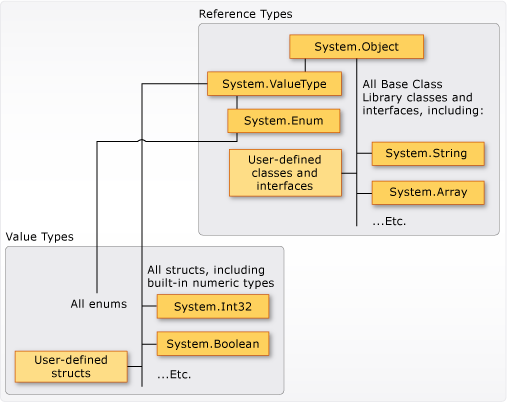
\includegraphics[width=140mm, height=100mm]{../img/value-reference-types-common-type-system}
%\caption{C\# type system \cite{online:cSharpTypeSystem}.}
%\label{img01:typeSystem}
%\end{figure}

\section{Roslyn}

\change{Overview of compilation pipeline}
\change{Binder}
\change{OverloadResolution}
\change{MethodTypeInferrer}
\change{NullableWalker}
\change{Dynamic biding vs. runtime binding}

\section{Hindley-Millner type inference}

\change{Hindley-Millner type system}
\change{Set of rules}
\change{Restriction and possible extensions}

\section{Rust type inference}

\change{Rust type system}
\change{Type inference context}
\change{Type inference across multiple statement}
\change{Constructor type inference}

\section{Github issues}

\change{Mention related Github issues and csharplang repo.}
\change{Roslyn and csharplang repo}
\change{Proposal champions}
\change{Related issues}
